%===============================================================================
% ifacconf.tex 2022-02-11 jpuente  
% 2022-11-11 jpuente change length of abstract
% Template for IFAC meeting papers
% Copyright (c) 2022 International Federation of Automatic Control
%===============================================================================
\documentclass{ifacconf}

% \usepackage{hyperref}
\usepackage{graphicx}      % include this line if your document contains figures
\usepackage{natbib}        % required for bibliography
\usepackage{comment}
\usepackage{amsmath}
\usepackage{amssymb}
\usepackage[dvipsnames]{xcolor}

\usepackage{subfig}
\usepackage{kotex}
\usepackage{tikz}

\usepackage{lipsum} % for dummy text
\usepackage{multirow}
\usepackage{multicol}

\usepackage{algorithm}
\usepackage{algpseudocode}

\usepackage{xurl}

% ============================================
%         GENERAL MACROS
% ============================================
\newcommand{\template}{template}
\newcommand{\KHCH}[1]{{\color{RoyalPurple} [KH: #1]}} % Kyunghwan's
\newcommand{\MSRY}[1]{{\color{Peach} [MS: #1]}} % Myeongseok's 
\newcommand\eg{\textrm{e.g.,\ }}
\newcommand\ie{\textrm{i.e.,\ }}
\definecolor{my_cyan}{rgb}{0.0, 1.0, 1.0}

\newcommand{\colorLine}[2]{[\tikz[baseline=(current bounding box.base)]{\draw[color=#1,
#2,line width=2pt] (0,3pt) -- (1.5em,3pt);}]}
% colors
% https://latexcolor.com % color list
\definecolor{airforceblue}{rgb}{0.36, 0.54, 0.66}
\definecolor{awesome}{rgb}{1.0, 0.13, 0.32}
\definecolor{darkcyan}{rgb}{0.0, 0.545, 0.545}
\newcommand{\ctxt}[2]{{\color{#1}{#2}\color{black}}}
\newcommand{\cred}[1]{{\ctxt{awesome}{#1}}}
\newcommand{\cblue}[1]{{\ctxt{airforceblue}{#1}}}

\begin{comment}
L2 Norm of Tracking Error:
C1: 2.0486
C2: 1.6893
C3: 6.8005
Improvement over C3:
C1: 69.88 %
C2: 75.16 %
\end{comment}

\newcommand{\oneErr}{{2.0486}}
\newcommand{\twoErr}{{1.6893}}
\newcommand{\threeErr}{{6.8005}}

\newcommand{\impOne}{{69.88}}
\newcommand{\impTwo}{{75.16}}

% ============================================
%         MATH MACROS
% ============================================
% \input{\template/macros/macros_math.tex}
\newcommand\R{\mathbb{R}}
\newcommand\N{\mathbb{N}}

\newcommand*{\mv}[1]{\boldsymbol{#1}} % my vector
\newcommand*{\mm}[1]{\boldsymbol{#1}} % my matrix
\newcommand*{\norm}[1]{\left\lVert #1 \right\rVert} % euclidean norm

\DeclareMathOperator{\myvec}{{vec}}       % vectorization
\DeclareMathOperator{\myproj}{{Proj}}   % projection
\DeclareMathOperator{\mysat}{{sat}}       % saturation
\DeclareMathOperator{\myrow}{{row}}       % row of a matrix
\DeclareMathOperator{\mycol}{{Col}}       % column of a matrix
\DeclareMathOperator{\mysym}{{sym}}       % symmetric part of a matrix
\DeclareMathOperator{\mydiag}{{diag}}     % diagonal matrix
\DeclareMathOperator{\mysign}{{sign}}     % sign function
\DeclareMathOperator{\mypoly}{{Poly}}     % polynomial

% ============================================
%         FRACTIONS
% ============================================
\newcommand\der{\mathrm d}
\newcommand*{\ddt}{
   \frac{\der}{\der t}
}
\newcommand*{\ddtt}{
   \tfrac{\der}{\der t}
}
\newcommand*{\ddttddtt}{
   \tfrac{\der^2}{\der t^2}
}
\newcommand*{\ddfrac}[2]{
   \frac{\der {#1}}{\der {#2}}
}
\newcommand*{\ddtfrac}[2]{
   \tfrac{\der {#1}}{\der {#2}}
}
\newcommand*{\ppfrac}[2]{
   \frac{\partial {#1}}{\partial {#2}}
}
\newcommand*{\pptfrac}[2]{
   \tfrac{\partial {#1}}{\partial {#2}}
}

%===============================================================================
\begin{document}
\begin{frontmatter}

\title{
   Vector-Space Optimization for Contraction Theory-Based Control Design: An Energy-Based Effective Space Approach
   \thanksref{footnoteinfo}
} 
% Title, preferably not more than 10 words.

\thanks[footnoteinfo]{
   This work was supported in part by the National Research Foundation of Korea (NRF) grant funded by the Korea government (MSIT) (RS-2025-00554087)
}

\author[First]{Myeongseok Ryu} 
\author[First]{Kyunghwan Choi} 
\author[Second]{Sesun You}

\address[First]{
   Korea Advanced Institute of Science and Technology (KAIST), 
   Daejeon 34051, South Korea (e-mail: \{dding\_98, kh.choi\}@kaist.ac.kr)}
\address[Second]{
   Incheon National University, 
   Incheon 22012, South Korea (e-mail: yousesun@inu.ac.kr)}

\begin{abstract}                % Abstract of 50--100 words
   In this paper, we propose a vector-space optimization framework for contraction theory-based control design.
   % Conventional contraction theory-based control design relies on matrix-space optimization, which suffers from computational complexity issues for high-dimensional systems.
   Conventional contraction theory-based feedback design methods typically require matrix-valued contraction metrics, which are obtained either over a prescribed domain in advance or through LMI-based optimization at each time instant.
   Although such approaches provide systematic stability certificates, their matrix-space formulation can limit real-time applicability as the system dimension increases and flexibility in handling nonlinear constraints, such as input saturation.
   To address these issues, we project the contraction condition onto the trajectory error vector space, and introduce the metric-weighted error vector as the optimization variable.
   This yields a lower-dimensional effective-space formulation that avoids solving for the full contraction metric online.
   Moreover, an energy-based constraint is introduced to resolve the scale ambiguity of condition-number minimization and to maintain sufficient control effort.
   The effectiveness and feasibility of the proposed method are validated through numerical simulations using the Lorenz system.
\end{abstract}

\begin{keyword}
   Contraction theory, 
   optimization-based control,
   % input saturation, 
   energy-based control
\end{keyword}

% e^T P e
% -> energy 

% M --> alpha
% e - > 0 ; 줄어들긴함
% e_1 - e_2 exp rate alpha

% sat
% x_d; dot x high; input sat
% x_d - x increase -> contracting no
% ->> 충분조건 안함
% ->> CBF 로 피해가기

% xd condition?
% reachability???? 

% M <-constraint 만족하는 M + 수축조건 하드에게

% 근사했을때 \hat M <- e 조건만족? 
% M(x, xd) x xd 

% ->> 필요조건
% ->> full CCM과 같아지나?

% y = M e 
% Y = M E = [y1, y2, y3] 
% E = [e, e_{k-1}, e_{k-2}]

% c(y_1) <= 0
% Y^T (..) Y + (..) Y + C <= 0

% \delta e^T M \delta e
% -> contracting
% full CCM 

\end{frontmatter}
%===============================================================================

\section{Introduction}

\subsection{Motivation}

Besides the traditional Lyapunov stability theory, contraction theory provides a powerful framework for analyzing nonlinear systems from an incremental stability perspective.
Rather than studying convergence to a fixed equilibrium point, contraction theory examines whether infinitesimally close trajectories exponentially converge to each other under a Riemann metric, called a contraction metric \cite{LOHMILLER:1998aa}.
Based on this differential viewpoint, contraction theory has been extended to control and observer design, as reviewed in \cite{Tsukamoto:2021aa} and \cite{Bernard:2022aa}, respectively.

Specifically, control contraction metrics (CCMs) have been developed for feedback control design, providing global stability certificates by introducing convex feasibility problems \cite{Manchester:2014aa,Manchester:2017aa}.
In CCM-based control design, the contraction metric is typically constructed over a prescribed operating domain in advance, often through gridding, sampling, or finite-dimensional parameterization.
Using the obtained contraction metric, a feedback control law can be obtained by integrating a differential feedback law along a shortest path, called a geodesic, between the current state and the desired trajectory.

However, enforcing the contraction condition over an entire operating domain can be computationally demanding, and the burden can increase rapidly with the dimension and size of the operating region.
Moreover, the resulting metric is tied to the selected domain and discretization, so the design may need to be repeated when the operating region or system configuration changes.
These limitations motivate step-wise formulations that compute a contraction metric at each time instant, rather than constructing a global metric over the full domain offline.

Among recent developments in contraction theory-based control, Tsukamoto {\etal} proposed ConVex optimization-based Steady-state Tracking Error Minimization (CV-STEM) \cite{Tsukamoto:2019aa}.
CV-STEM is a systematic framework for contraction metric calculation that solves a linear matrix inequality (LMI) optimization problem to minimize the steady-state tracking error bound in the presence of bounded disturbances.
Unlike conventional CCM-based approaches that construct a global metric over a prescribed domain offline, CV-STEM computes the contraction metric at each time instant for the current state and desired trajectory.
The framework has been developed in both state-dependent coefficient (SDC)-based and CCM-based formulations \cite{Tsukamoto:2021aa}.
In the SDC-based formulation, the error dynamics are linearized using the SDC formulation as a linear parameter-varying (LPV) system and the contraction metric is directly applied as a feedback gain for the trajectory error.
In the CCM-based formulation, the contraction metric defines a geodesic between the current state and the desired trajectory, along which a differential feedback law is integrated to compute the actual control input.
CV-STEM has demonstrated its effectiveness and has been extended to various systems, including stochastic systems \cite{Tsukamoto:2021ad} and uncertain systems \cite{Tsukamoto:2021af}.

Despite these advances, CV-STEM still relies on matrix-space LMI optimization when the metric is computed online.
For an $n$-dimensional system, the contraction metric is an $n\times n$ symmetric positive definite matrix, and thus the number of independent matrix variables grows quadratically with the system dimension \cite{Boyd:2004aa}.
This matrix-valued decision variable can limit the scalability of step-wise contraction-metric computation as the system dimension increases.
Although some studies have proposed offline approximation of the contraction metric using deep neural networks (DNNs) \cite{Tsukamoto:2021ae,Tsukamoto:2021ac}, it is desirable to reduce the dimension of the online optimization variable without relying on offline approximation.

Moreover, there has been limited consideration of input saturation in conventional contraction theory-based control design, which limits the practical applicability of the method.
For instance, in \cite{Tsukamoto:2019aa}, the input saturation constraint is considered in a conservative manner by limiting the maximum norm of the control input, rather than directly incorporating the contraction metric into the LMI framework.
This may lead to the infeasibility of the optimization problem when the input saturation constraint is tight.
In addition, if the input saturation effect is not properly handled, the system performance may degrade significantly or even become unstable \cite{Ryu:2025aa}.

Another issue arises from the condition-number objective used in LMI optimization problems.
Since the steady-state tracking-error bound is proportional to the condition number of the contraction metric, the objective is to minimize the condition number.
However, the condition number is invariant under positive scaling of the metric, and therefore condition-number minimization alone does not uniquely determine the magnitude of the metric.
Consequently, the resulting feedback gain and control effort can become ambiguous: different scalings of the metric can yield the same condition number but different control magnitudes.
This motivates the introduction of an additional constraint that specifies the required metric-induced energy while retaining the error-bound interpretation of condition-number minimization.

% There is also the issue of an ill-posed problem in the objective function minimizing the condition number of the contraction metric, which is proportional to the steady-state error bound.
% Since the condition number is scale-invariant, there exist an infinite number of solutions for the contraction metric that yield the same condition number.
% In conventional approaches, this issue has been tackled by introducing a scaling parameter for the contraction metric and tuning it with weighting factors in the objective function \cite{Tsukamoto:2019aa,Tsukamoto:2021ae}.
% However, this approach may determine insufficient control effort to achieve the desired trajectory or lead to excessive control effort.

Motivated by these observations, this paper proposes an effective-space optimization framework for contraction theory-based control design.
Instead of optimizing directly over the full matrix-valued contraction metric, we exploit the fact that the metric appears in the feedback law through its action on the trajectory error.
By introducing the metric-weighted error vector, the contraction condition is projected onto the instantaneous error direction and converted into a vector-space optimization problem.
This reduces the online decision variable from a matrix-valued metric to a vector-valued effective-space variable.
In addition, an energy-based constraint is introduced to resolve the scale ambiguity of condition-number minimization and to maintain sufficient control effort.

% \cred{이거도 마찬가지임}
% On the other hand, by formulating the problem in vector space rather than matrix space, flexibility in handling various constraints, including nonlinear input and state constraints, can be improved.
% In addition, the dependency of computational complexity on the system dimension can be alleviated.
% If the contraction metric is utilized as a feedback gain for the trajectory error, the contraction metric can be projected onto the trajectory error vector space.
% This allows us to simplify the contraction metric calculation from matrix-space optimization to vector-space optimization within a lower-dimensional effective space.

% To the best of our knowledge, there has been no previous work that projects the contraction constraints onto a vector space to reduce the dependency on the system dimension for contraction metric calculation.
% Moreover, input saturation has not been actively considered in conventional contraction theory-based control design.
% Hence, the main objective of this paper is to simplify the contraction metric calculation from matrix-space optimization to vector-space optimization, while also incorporating the input saturation constraint and maintaining sufficient control effort.

\subsection{Contributions}

The main contributions of this paper are:
\begin{itemize}
   \item A vector-space optimization framework is proposed by projecting the contraction condition onto the trajectory error direction and using the metric-weighted error vector as the decision variable;
   \item The proposed formulation reduces the online decision variable from a matrix-valued contraction metric to a vector-valued effective-space variable, thereby improving the scalability of step-wise contraction-metric computation;
   \item An energy-based constraint is introduced to resolve the scale ambiguity of condition-number minimization and to maintain sufficient control effort; and
   \item The feasibility and performance of the proposed framework are demonstrated through numerical simulations on the Lorenz system.

   % \item The contraction metrics can be calculated in a lower-dimensional effective space by projecting the contraction constraints onto the trajectory error vector space. This significantly reduces the computational complexity of the LMI framework for contraction metric calculation, enabling real-time implementation;
   % \item The scale-invariance issues of the objective function minimizing the condition number of the contraction metric are resolved by introducing energy-based constraints to obtain locally optimal solutions and maintain sufficient control effort;
   % \item A convex input saturation constraint is incorporated into the proposed optimization framework, which handles the practical limitations of actuators; and
   % \item The robust feasibility of the proposed method is enhanced by introducing slack variables to relax the energy-based constraints, thereby avoiding infeasibility due to the input saturation constraint.
\end{itemize}

\subsection{Paper Organization}

The remainder of this paper is organized as follows.
Section \ref{sec:preliminaries} reviews the preliminaries of contraction theory.
Section \ref{sec:problem} formulates the problem of contraction theory-based control design.
Section \ref{sec:conv:lmi} discusses the conventional LMI framework for contraction metric calculation and its limitations.
Section \ref{sec:main:results} presents the proposed vector-space optimization framework for contraction metric calculation and provides an illustrative example.
Section \ref{sec:validation} validates the proposed method through numerical simulations.
Finally, Section \ref{sec:conclusion} concludes the paper.

\section{Preliminaries} \label{sec:preliminaries}

Before presenting the proposed method, we first review contraction theory and related theorems.
A detailed explanation of contraction theory can be found in \cite{LOHMILLER:1998aa,Manchester:2017aa,Tsukamoto:2021aa}.

\subsection{Contraction Property and Contraction Metric} \label{sec:sub:contraction}

Consider the following nonlinear system:
\begin{equation} \label{eq:pre:sys}
   \ddtt\mv{x}
   =
   \mv{f}(\mv{x},t)
   ,
\end{equation}
where $\mv{x}\in\R^n$ denotes the state variables and $\mv{f}:=\mv{f}(\mv{x},t)$ denotes the nonlinear system function.
Additionally, consider the differential dynamics of the system \eqref{eq:pre:sys}, which is represented as 
$
   \ddtt{\delta\mv{x}}
   =
   \pptfrac{\mv{f}}{\mv{x}} \delta\mv{x}
$
, \cite[Chap 4]{Kirk:2004aa}.

According to \cite{LOHMILLER:1998aa}, the system \eqref{eq:pre:sys} is said to be \textit{contracting}, \ie all trajectories converge incrementally exponentially to a unique trajectory, if the following condition holds:
\begin{equation} \label{eq:pre:contraction:condition}
   \ddtt\mm{M} 
   + 
   2\mysym
   \left(
      \mm{M} \pptfrac{\mv{f}}{\mv{x}}
   \right) 
   \preceq 
   -2\alpha\mm{M}
   ,
\end{equation}
where $\mm{M}$ denotes the \textit{contraction metric}, $\alpha\in\R_{>0}$ denotes the \textit{contraction rate}, and $\mysym(\mm A):=\tfrac{1}{2}(\mm A+\mm A^\top)$.
The contraction metric $\mm{M}$ is a symmetric positive definite matrix satisfying $\overline{m}\mm{I}_n\succeq\mm{M}\succeq\underline{m}\mm{I}_n$ with $\overline{m},\underline{m}\in\R_{>0}$.

Notably, the initial conditions are exponentially forgotten in a contracting system \cite{LOHMILLER:1998aa}.

\subsection{Perturbed Contracting System} \label{sec:sub:contraction:perturbed}

If the system \eqref{eq:pre:sys} is subjected to bounded disturbances, it can be expressed as follows:
\begin{equation} \label{eq:pre:sys:perturbed}
   \ddtt\mv{x}
   =
   \mv{f}(\mv{x},t)
   +
   \mv{d}(t)
   , 
\end{equation}
where $\mv{d}(t)\in\R^n$ denotes the external disturbances with $\norm{\mv{d}(t)}\leq \overline{d}$, where $\overline{d}\in\R_{>0}$.

The following theorem states that all solutions of the perturbed system \eqref{eq:pre:sys:perturbed} exponentially converge to a bounded ball around the solution of the nominal system \eqref{eq:pre:sys}.
\begin{thm} \label{thm:contraction:perturbed}
   If the system \eqref{eq:pre:sys} is contracting with the contraction metric $\mm{M}$ satisfying the condition \eqref{eq:pre:contraction:condition}, the path integral $V_l(\mv{q},\delta\mv{q},t)=\int_{\mv{\xi}_1}^{\mv{\xi}_2}\norm{\mm{\Theta}(\mv{q},t)\delta\mv{q}}$, where $\mm{\Theta}(\mv{q},t):=\mm{M}^{1/2}$, and $\mv{\xi}_1$ and $\mv{\xi}_2$ are the solutions of \eqref{eq:pre:sys} and \eqref{eq:pre:sys:perturbed}, respectively, and $\mv{q}$ is the virtual state variable, exponentially converges to a bounded ball. 
   Specifically, the following inequality for a bounded error ball of the solutions of \eqref{eq:pre:sys} and \eqref{eq:pre:sys:perturbed} holds:
   \begin{equation}
      \norm{\mv\xi_1(t)-\mv\xi_2(t)}
      \le
      \tfrac{V_{l}(0)}{\sqrt{\underline{m}}}
      \exp(-\alpha t)
      +
      \tfrac{\overline d}{\alpha}
      \sqrt{\chi}
      (1-\exp(-\alpha t))
      ,
   \end{equation}
   where $\chi:=\overline{m}/\underline{m}$ denotes the condition number of $\mm{M}$, yielding a steady-state error bound of $\tfrac{\overline d}{\alpha}\sqrt{\chi}$.
\end{thm}

\begin{pf}
   See the proof of Theorem 2.4 in \cite{Tsukamoto:2021aa}.
\end{pf}

\section{Problem Formulation} \label{sec:problem}

Let us consider the following nonlinear system:
\begin{equation} \label{eq:sys}
   \begin{aligned}   
      \ddtt{\mv{x}}
      =&
      \mv{f}(\mv{x},t)
      +
      \mm{B}(\mv{x},t)
      \mysat(\mv{u})   
      +
      \mv{d}(t)
      ,
   \end{aligned}
\end{equation}
where $\mv{x}\in\R^n$ and $\mv{u}\in\R^m$ denote the state variables and control inputs, respectively; $\mv{d}:=\mv{d}(t)\in\R^n$ denotes the bounded external disturbances, \ie $\norm{\mv{d}} \leq \overline{d}$; and $\mv{f}(\mv{x},t)$ and $\mm{B}(\mv{x},t)$ denote the system functions.
The input saturation function is denoted by $\mysat(\cdot)$ and can be defined as any physically feasible function.

The system \eqref{eq:sys} is assumed to satisfy the following assumptions:

\begin{assum}[Smoothness of System Functions] \label{assum:sys:smooth}
   The system functions $\mv{f}(\mv{x},t)$ and $\mm{B}(\mv{x},t)$ are smooth in $\mv{x}$ and $t$, implying Lipschitz continuity.
\end{assum}

\begin{assum}[Full row rank of $\mm{B}$] \label{assum:sys:B}
   The control effectiveness matrix $\mm{B}(\mv{x},t)$ has full row rank for all $\mv{x}\in\R^n$ and $t\in\R_{\geq 0}$.
\end{assum}


We assume that a desired control input $\mv{u}_d\in\R^m$ is pre-designed to achieve the desired trajectory $\mv{x}_d\in\R^n$ under ideal conditions, \ie $\mv{d}=0$, by simulating the following desired system:
\begin{equation} \label{eq:sys:desired}
   \ddtt\mv{x}_d   =
   \mv{f}(\mv{x}_d, t)   
   +
   \mm{B}(\mv{x}_d,t) \mv{u}_d
   .
\end{equation}

The error dynamics between the system \eqref{eq:sys} and the desired system \eqref{eq:sys:desired} can be expressed as follows:
\begin{equation} \label{eq:error:dyn:1}
   \begin{aligned}
      \ddtt\mv{e}
      =&
      \mv{f}-\mv{f}_d
      + \mm{B} \mysat(\mv{u})
      - \mm{B}_d \mv{u}_d
      + \mv{d}
      ,
   \end{aligned}
\end{equation}
where $\mv{e}:=\mv{x}-\mv{x}_d$ denotes the trajectory error vector, and the arguments of $\mv{f}$, $\mv{f}_d$, $\mm{B}$, and $\mm{B}_d$ are omitted for brevity.
Using the SDC formulation \cite{Dani:2015aa}, \ie 
$
   \mathbb{A}
   :=
   \mathbb{A}(\mv{x},\mv{x}_d)
   =
   \int_0^1 
   \left[
      \pptfrac{\overline{\mv{f}}}{\mv{x}}
   \right]
   \big(
      c \mv{x} + (1-c) \mv{x}_d
   \big)
   \,\der c
   ,
$ 
where $\overline{\mv{f}}:=\mv{f}-\mv{f}_d+(\mm{B}-\mm{B}_d)\mv{u}_d$, the error dynamics \eqref{eq:error:dyn:1} can be represented as follows:
\begin{equation} \label{eq:error:dyn:2}
   \begin{aligned}
      \ddtt\mv{e}
      =&
      \underbrace
      {
         \mv{f}-\mv{f}_d
         +
         (
            \mm{B} 
            - \mm{B}_d 
         ) \mv{u}_d
      }_{= \mathbb{A}(\mv{x},\mv{x}_d) \mv{e}}
      % \\
      % &
      + \mm{B} 
      (
         \mv{u} - \mv{u}_d
      )
      + \mm{B} \mv{\phi}(\mv{u}) + \mv{d}
      \\
      =&
      \mathbb{A} \mv{e}
      + \mm{B} 
      (\mv{u} - \mv{u}_d)
      + \mm{B} \mv{\phi}(\mv{u}) + \mv{d}
      ,
   \end{aligned}
\end{equation}
where $\mv{\phi}(\mv{u}):=\mysat(\mv{u}) - \mv{u}$ denotes the input saturation effect.

To simplify the control design, we use the following state feedback control law:
\begin{equation} \label{eq:control:law}
   \mv{u}
   =
   \mv{u}_d
   -
   \mm{R}^{-1} \mm{B}^\top \mm{M}
   % ( 
   %    \mv{x} - \mv{x}_d
   % )
   \mv{e}
   ,
\end{equation}
where $\mm{R}\in\R^{m\times m}$ denotes a positive definite weighting matrix for the control input.
Substituting the control law \eqref{eq:control:law} into the error dynamics \eqref{eq:error:dyn:2}, we obtain:
\begin{equation} \label{eq:error:dyn:3}
   \ddtt\mv{e}
   \!=\!
   \left(
      \mathbb{A} - \mm{B} \mm{R}^{-1} \mm{B} ^\top \mm{M}
   \right)
   \mv{e}
   + \mm{B} \mv{\phi}(\mv{u}) + \mv{d}
   .
\end{equation}

Finally, the control objective is to obtain the contraction metric $\mm{M}$ in \eqref{eq:control:law} which guarantees that the system \eqref{eq:sys} is contracting with respect to the desired trajectory $\mv{x}_d$ in the presence of input saturation and external disturbances.

\section{Conventional Matrix-Space Formulation} \label{sec:conv:lmi}

% In \cite{Tsukamoto:2019aa,Tsukamoto:2021ae}, Tsukamoto {\etal} proposed ConVex optimization-based Steady-state Tracking Error Minimization (CV-STEM) to obtain the contraction metric $\mm{M}$ in the control input \eqref{eq:control:law} by formulating an LMI optimization problem.

% In this section, we review the CV-STEM framework proposed by Tsukamoto {\etal} in \cite{Tsukamoto:2021aa}, and discuss its potential limitations.
% It should be noted that the input saturation effect is not explicitly handled in CV-STEM framework.

To apply Theorem \ref{thm:contraction:perturbed}, define the systems \eqref{eq:pre:sys} and \eqref{eq:pre:sys:perturbed} as \eqref{eq:sys} with $\mv{d}=\mv{0}$ and \eqref{eq:sys}, respectively, and the virtual $\mv{q}$-system as $\ddtt(\mv{q}-\mv{x}_d)=(\mathbb{A}-\mm{B}\mm{R}^{-1}\mv{B}^\top\mm{M})(\mv{q}-\mv{x}_d)+\mu\mv{d},\ \mu\in[0,1]$, whose solutions are denoted by $\mv{q}(\mu=0,t)=:\mv{\xi}_1$ and $\mv{q}(\mu=1,t)=:\mv{\xi}_2$, respectively.
Then, neglecting the input saturation effect, the steady-state error bound between the system \eqref{eq:sys} and the desired system \eqref{eq:sys:desired} can be reduced by minimizing the condition number $\chi$ of the contraction metric $\mm{M}$ proportionally, as follows:
% \begin{equation} \label{eq:err:ss}
$
   \lim_{t\to\infty}
   \norm{\mv{e}(t)}
   =
   \overline{d}
   \tfrac{\sqrt{\chi}}{\alpha}
$.
% \end{equation}
The contraction constraint \eqref{eq:pre:contraction:condition} in Theorem \ref{thm:contraction:perturbed}, which should be satisfied by the contraction metric $\mm{M}$, can be expressed for the error dynamics \eqref{eq:error:dyn:3} as follows:
\begin{equation} \label{eq:cstr:ctrc}
   \ddtt\mm{M}
   +
   2\mysym
   \left(
      \mm{M}
      \mathbb{A}
   \right)
   - 
   2
   \mm{M}\mm{B}\mm{R}^{-1}\mm{B}^\top\mm{M}
   \preceq
   -2\alpha \mm{M}
   .
\end{equation}

Using the variable transformation $\mm{M}=:\mm{W}^{-1}$, the following LMI optimization problem can be formulated:
\begin{equation} \label{eq:opt:conv:lmi}
   \begin{matrix}
      \min_{
         \overline{\mm{W}},\chi,\nu
         } 
      \chi + \lambda \nu
      \\ 
      \vspace{-.2cm}
      \\
      \text{s.t. }
      \begin{cases}
         -
         \ddtt\overline{\mm{W}}
         +
         2\mysym(
            \mathbb{A}\overline{\mm{W}}
         )
         -
         2\nu\mm{B}\mm{R}^{-1} \mm{B}^\top 
         \preceq
         -2\alpha\overline{\mm{W}}
         ,
         \\
         \mm{I}_n
         \preceq
         \overline{\mm{W}}
         \preceq
         \chi \mm{I}_n
         ,
      \end{cases}
   \end{matrix}
\end{equation} 
where $\overline{\mm{W}}:=\nu\mm{W}$ and $\nu\in\R_{>0}$ is a penalty term for the 2-norm of $\mm{M}$.
Using $\lambda\in\R_{>0}$, the magnitude of $\mm{M}$ can be adjusted by $\nu$.
Since the LMI optimization problem \eqref{eq:opt:conv:lmi} is convex, a global optimal solution can be obtained.

However, since the optimization variable is the inverse of $\mm{M}$, the input saturation constraint is not explicitly considered in the LMI optimization problem \eqref{eq:opt:conv:lmi}.
In \cite{Tsukamoto:2019aa}, the input saturation constraint is considered in a conservative manner by limiting the maximum norm of the control input, rather than directly incorporating $\mm{M}$, \ie $\norm{\mv{u}}\leq \overline{u}$ where $\overline{u}\in\R_{>0}$.
This makes the optimization problem \eqref{eq:opt:conv:lmi} potentially infeasible when the norm constraint of the input is too conservative.
In addition, Theorem~\ref{thm:contraction:perturbed} cannot be directly applied to the system \eqref{eq:sys} with input saturation, since $\mv{\phi}(\mv{u})=\mysat(\mv{u})-\mv{u}$ is not considered a bounded disturbance.

From the perspective of scalability, the number of independent decision variables of \eqref{eq:opt:conv:lmi} grows quadratically with the system dimension.
% From the perspective of computational complexity, the complexity of solving the LMI optimization problem \eqref{eq:opt:conv:lmi} is quadratically dependent on the dimension.
In addition, the LMI framework limits flexibility in handling various constraints, including nonlinear input and state constraints.
Thus, these issues should be resolved for practical real-time implementation.

Motivated by these observations, the next section develops a vector-space formulation that directly optimizes the metric-weighted error vector rather than the full matrix-valued contraction metric.

% In conclusion, although CV-STEM provides a systematic framework for contraction metric calculation in an LMI framework, several issues remain to be resolved for practical real-time implementation.

% \cred{
% \begin{rem} \label{rem:scale:invariance}
%    A potential implementation issue arises when the scaling variable $\nu$ is treated as time-varying in the discretized derivative term.
%    % There exists a severe problem formulation issue in the conventional LMI framework.
%    In the formulation, $\ddtt\overline{\mm{W}}=\ddtt(\nu\mm{W})$ is considered the same as $\nu\ddtt(\mm{W})$, which does not hold since $\nu$ is also a decision variable.
%    Thus, the conventional LMI framework's solutions may determine $\overline{W}$ and $\chi$ to be $\mm{I}_n$ and $1$, respectively, and modify $\nu$ only, leading to potential violation of the contraction constraint \eqref{eq:cstr:ctrc}.
% \end{rem}
% }

\section{Main Results} \label{sec:main:results}

\subsection{Projection of Contraction Condition}

In this section, we present the proposed vector-space optimization framework.
We project the contraction condition \eqref{eq:cstr:ctrc} onto the trajectory error vector space by pre- and post-multiplying it by $\mv{e}^\top$ and $\mv{e}$, respectively, as follows:
\begin{equation} \label{eq:cstr:ctrc:proj}
   -
   2
   \mv{y}^\top 
   \left(
      \mm{B} 
      \mm{R}^{-1} 
      \mm{B}^\top
   \right)
   \mv{y}
   +
   \mv{e}^\top
   \!
   \left(
      \tfrac{1}{T_s}+2\alpha
      +
      2\mathbb{A}^\top
   \!
   \right)
   \mv{y}
   -
   \tfrac{\mv{e}^\top \mm{M}_{\rm{pre}} \mv{e}}{T_s}
   \le 0
   ,
\end{equation}
where $\mv{y}:=\mm{M}\mv{e}$ denotes a metric-weighted error vector, serving as a new optimization variable.
For discrete-time implementation, $\ddtt\mm{M}$ is approximated as $\tfrac{1}{T_s}(\mm{M}-\mm{M}_{\rm{pre}})$, where $T_s$ denotes the sampling time and $\mm{M}_{\rm{pre}}$ denotes the contraction metric obtained at the previous time step.

To justify the proposed approach, we first present the following theorem that provides a sufficient condition of the projected contraction condition \eqref{eq:cstr:ctrc:proj} to guarantee the full contraction condition \eqref{eq:cstr:ctrc}.

\begin{thm} \label{thm:proj:ctrc:suff}
   For the system \eqref{eq:sys} satisfying Assumption~\ref{assum:sys:B} with the control law \eqref{eq:control:law}, the projected contraction condition \eqref{eq:cstr:ctrc:proj} is necessary for the full contraction condition \eqref{eq:cstr:ctrc}.
   Furthermore, suppose that there exists a metric-weighted error vector $\mv y=\mm M\mv e$ satisfying \eqref{eq:cstr:ctrc:proj}.
   If the reconstructed matrix $\mm M$ from $\mv y$ has a sufficiently large error-directional metric scale $\mu$ and a sufficiently small condition number $\chi$, then the reconstructed matrix also satisfies the full contraction condition \eqref{eq:cstr:ctrc}.
\end{thm}

\begin{pf}

   \emph{Necessity.}

   If the full contraction condition \eqref{eq:cstr:ctrc} holds, then pre- and post-multiplying it by $\mv e^\top$ and $\mv e$ directly yields the projected condition \eqref{eq:cstr:ctrc:proj}.

   Therefore, the projected condition is necessary for the full contraction condition.

   \emph{Sufficiency.}

   Since the control effectiveness matrix $\mm{B}$ is full row rank matrix according to Assumption~\ref{assum:sys:B}, we have 
   \begin{equation}
      \mm{B}\mm{R}^{-1}\mm{B}^\top 
      \ge
      \sigma \mm{I}_n
      ,
   \end{equation}
   for some $\sigma\in\R_{>0}$.
   In addition, according to Assumption~\ref{assum:sys:smooth}, the SDC $\mathbb{A}$ is bounded such that $\norm{\mathbb{A}} \le \overline{A},$ for some $\overline{A}\in\R_{>0}$.

   The error-directional metric scale $\mu$ can be defined as follows:
   \begin{equation}
      \mu
      :=
      \frac{\mv{e}^\top\mm{M}\mv{e}}{\mv{e}^\top\mv{e}}
      .
   \end{equation}
   By the definition of $\mm{M}$, the following inequality holds:
   \begin{equation} \label{eq:mu:bounds}
      \underline{m}
      \le
      \mu
      \le
      \overline{m}
      \implies
      \tfrac{\mu}{\chi}
      \le 
      \underline{m}
      ,\ 
      \overline{m}
      \le
      \mu \chi
      ,\ 
      1
      \le 
      \chi 
      .
   \end{equation}
   % \mu/\underline{m} \le \chi
   % \mu / \chi \le \underline{m}
   % 1/\chi \le \mu/\overline{m}
   % \overline{m} \le \mu \chi

   Each term of the projected contraction condition \eqref{eq:cstr:ctrc:proj} can be conservatively upper-bounded as follows:
   \begin{align}
      -2
      \norm{
         \mv{y}^\top 
         \!
         \left(
         \!
            \mm{B} 
            \mm{R}^{-1} 
            \mm{B}^\top
         \!
         \right)
         \mv{y}
      }
      &\le
      -2\sigma\underline{m}^2
      \norm{\mv{e}}^2
      \\
      \norm{
         \mv{e}^\top
         \!
         \left(
            \tfrac{1}{T_s}+2\alpha
            +
            2\mathbb{A}^\top
         \!
         \right)
         \mv{y}
      }
      &\le
      \left(
         \tfrac{1}{T_s}
         +
         2
         \left(
            \alpha
            +
            \overline{A}
         \right)
      \right)
      \overline{m}
      \norm{\mv{e}}^2
      ,
      \\
      -
      \norm{
         \tfrac{\mv{e}^\top \mm{M}_{\rm{pre}} \mv{e}}{T_s}
      }
      &\le
      -
      \tfrac{1}{T_s}\underline{m}
      \norm{\mv{e}}^2
      . 
   \end{align}
   By substituting the above inequalities into \eqref{eq:cstr:ctrc:proj}, we have
   \begin{equation}
      \left(
      -2\sigma\underline{m}^2
      % \norm{\mv{e}}^2
      +
      \left(
         \tfrac{1}{T_s}
         +
         2
         \left(
            \alpha
            +
            \overline{A}
         \right)
      \right)
      \overline{m}
      -\tfrac{1}{T_s}\underline{m}
      \right) 
      \norm{\mv{e}}^2
      \le 0
      .
   \end{equation}
   Additionally, invoking \eqref{eq:mu:bounds}, the above inequality can be further rearranged as follows:
   \begin{equation}
      -2\sigma \tfrac{\mu^2}{\chi^2}
      +
      \left(
         \tfrac{1}{T_s}
         +
         2
         \left(
            \alpha
            +
            \overline{A}
         \right)
      \right)
      \mu \chi
      -\tfrac{1}{T_s}\tfrac{\mu}{\chi}
      \le 0
      .
   \end{equation}
   
   Finally we have the following sufficient condition for the full contraction condition \eqref{eq:cstr:ctrc}:
   \begin{align} \label{eq:suff:cond:mu}
      \mu\ge
      &
      \tfrac{1}{2\sigma}
      \left(
         2(\alpha+\overline{A})\chi^3
         +
         \tfrac{1}{T_s}
         \left(
            \chi^3
            -
            \chi
         \right)
      \right)
      .
   \end{align}
   The right-hand side of \eqref{eq:suff:cond:mu} is monotonically increasing with respect to $\chi$ for $\chi\ge 1$.
   Thus, if $\mu$ is sufficiently large and $\chi$ is sufficiently small such that the inequality \eqref{eq:suff:cond:mu} holds, the full contraction condition \eqref{eq:cstr:ctrc} is guaranteed.

\end{pf}

\subsection{Vector-Space Optimization Framework} \label{sec:sub:vector:space:opt}

According to Theorem~\ref{thm:proj:ctrc:suff}, the following optimization problem can be formulated, as follows:
\begin{subequations} \label{eq:opt:main}
   \begin{align}
      \min_{
         \mv{y},s
         } 
         \quad &
      \norm{\mv{y}}\norm{\mv{e}} - \mv{y}^\top \mv{e}
      % J(\mv{y})
      +
      \lambda s
      \label{eq:opt:main:obj}
      \\
      \text{subject to} 
      \quad &
      % \begin{cases}
         \eqref{eq:cstr:ctrc:proj}
         ,
         \label{eq:opt:main:ctrc:proj}
         \\ &
         \left(
            \mv{e}^\top \mv{y} 
            -
            \mu \mv{e}^\top \mv{e}
         \right)^2
         \le
         (\epsilon + s) \norm{\mv{e}}^2
         ,
         \label{eq:opt:main:energy}
         \\ &
         c(\mv{y}) \le 0
         ,
         \label{eq:opt:main:sat}
      % \end{cases}
   \end{align}
\end{subequations}
where $s,\epsilon\in\R_{\ge0}$ denote the slack variable and the allowable small energy variation, respectively of the energy-based constraint \eqref{eq:opt:main:energy} which will be explained later; $\lambda\in\R_{>0}$ denotes the penalty term for the slack variable $s$ and $c(\cdot)$ denotes input constraints, which can be designed to handle the input saturation effect.

The objective function \eqref{eq:opt:main:obj} is designed to minimize the angle between $\mv{y}$ and $\mv{e}$, which is equivalent to minimizing the condition number of the contraction metric $\mm{M}$.
Additionally, the last term in \eqref{eq:opt:main:obj} is a penalty term for the slack variable $s$ which will be explained later.

Imposed constraints include the projected contraction constraint \eqref{eq:opt:main:ctrc:proj}, the energy-based constraint \eqref{eq:opt:main:energy}, and the input saturation constraint \eqref{eq:opt:main:sat}.

The energy-based constraint \eqref{eq:opt:main:energy} is designed to prescribe the error-directional metric scale by enforcing 
$\mv e^\top\mv y\approx\mu\mv e^\top\mv e$; since $\mv y=\mm M\mv e$, this corresponds to 
$\mv e^\top\mm M\mv e/\mv e^\top\mv e\approx\mu$.
According to Theorem~\ref{thm:proj:ctrc:suff}, a sufficiently large error-directional metric scale, together with a sufficiently small condition number, promotes satisfaction of the full contraction condition \eqref{eq:cstr:ctrc}.
However, due to the input saturation constraint \eqref{eq:opt:main:sat}, the projected contraction constraint \eqref{eq:opt:main:ctrc:proj} may conflict with the input saturation constraint \eqref{eq:opt:main:sat}, leading to potential infeasibility of the optimization problem \eqref{eq:opt:main}.
To resolve this issue, the slack variable $s$ is introduced to relax the energy-based constraint.

The input saturation constraint \eqref{eq:opt:main:sat} can be designed to directly handle the input saturation effect by defining $c(\mv{y})$ to represent the admissible input set induced by the saturation function $\mysat(\cdot)$.

After the optimization, the contraction metric $\mm{M}$ can be retrieved while maintaining the condition number and the relationship $\mv{y}=\mm{M}\mv{e}$ as follows:
\begin{equation} \label{eq:retrive:mm}
   \mm{M}
   =
   \tfrac{1}{\sqrt{\chi}}
   \mydiag
   \left(
      \begin{pmatrix}
         \sqrt{\chi}, 1, \ldots, 1, \tfrac{1}{\sqrt{\chi}}
      \end{pmatrix}
   \right)
   \cdot
   \tfrac{1}{\norm{\mv{e}}\norm{\mv{y}}}
   ,
\end{equation}
where $\chi=\tfrac{1+\sin(\theta)}{1-\sin(\theta)}$ denotes the minimum condition number of $\mm{M}$ when the angle $\theta$ between $\mv{y}$ and $\mv{e}$ is given.

% In summary, the proposed formulation replaces the online search over a matrix-valued metric with the optimization of the feedback-relevant metric action $\mv y=\mm M\mv e$.
% The obtained vector $\mv y$ directly determines the constrained feedback input, while a positive definite matrix $\mm M$ satisfying $\mm M\mv e=\mv y$ is reconstructed for evaluating the projected condition and for use in the subsequent time step.
% Thus, the proposed framework should be interpreted as a projected contraction-based design that prioritizes scalable computation and direct input-constraint handling, while recovering the full contraction condition when the sufficient metric-scale and condition-number conditions in Theorem~\ref{thm:proj:ctrc:suff} are satisfied.

In conclusion, instead of solving the matrix-space optimization problem \eqref{eq:opt:conv:lmi}, the proposed method solves the vector-space optimization problem \eqref{eq:opt:main} to obtain the projected contraction metric $\mv{y}$.
After that, to obtain the contraction metric $\mm{M}$ for the control law \eqref{eq:control:law} and $\mm{M}_{\rm{pre}}$ in \eqref{eq:cstr:ctrc}, the contraction metric $\mm{M}$ is retrieved using \eqref{eq:retrive:mm}.
   
The overall procedure of the proposed method is summarized in Algorithm~\ref{alg:alg:1}, in which the optimization problem \eqref{eq:opt:main} is solved at each time step.

\begin{algorithm}[!t]
   \caption{Proposed controller} \label{alg:alg:1}
   \begin{algorithmic}[1]
      \State \textbf{Initialize:} $\mv{y}_0=\mv{1}_{n\times 1}$, $s_0=0$, $\mm{M}_{0}=\mu\mm{I}_n$
      \For{$k = 1 $ to $\infty$}
            \State Get current $\mv{x}_k$, $\mv{x}_{d,k}$, $\mv{u}_{d,k}$ and $\mv{e}_k$
            \State Assign $\mv{y}_k \leftarrow \mv{y}_{k-1}$, $s_k \leftarrow s_{k-1}$ for warm-start
            \State Solve \eqref{eq:opt:main} to get optimal $\mv{y}_k$ and $s_k$
            \State Calculate $\mm{M}_{k}$ using $\mv{y}_k$ and $\mv{e}_k$ using \eqref{eq:retrive:mm}
            \State Apply the control law \eqref{eq:control:law} using $\mm{M}_{k}$
      \EndFor
   \end{algorithmic}
\end{algorithm}

\subsection{Illustrative Example in Two-Dimensional Space} \label{sec:sub:illustrative}

\begin{figure}[t]
   \centering
   
\includegraphics[width=0.99\linewidth]
   {
      figures/scene_first.drawio.pdf
   }
   \caption{
      Illustration of the optimization problem \eqref{eq:opt:main} in two-dimensional space; see Section \ref{sec:sub:illustrative} for details.
   }
\label{fig:scene:first}
\end{figure}

To facilitate geometric interpretation, the optimization problem \eqref{eq:opt:main} is illustrated in two-dimensional space in Fig.~\ref{fig:scene:first}.
The projected contraction condition \eqref{eq:opt:main:ctrc:proj} and the input saturation constraint \eqref{eq:opt:main:sat} restrict the feasible space of $\mv{y}$ to the outside of the blue line and the inside of the red line, respectively.
The green line represents the energy-based constraint \eqref{eq:opt:main:energy}, assuming that the allowable energy variation $\epsilon$ is approximately zero.

% Since the projected contraction constraint \eqref{eq:opt:main:ctrc:proj} is an ellipse-shaped concave function and the input saturation constraint \eqref{eq:opt:main:sat} is a convex function, there exist at most two intersection points of these constraints.
Without the input saturation constraint, the optimal solution is obtained at point (a) where \eqref{eq:opt:main:ctrc:proj} and \eqref{eq:opt:main:energy} are active, resulting in the minimum condition number of $\mm{M}$ and the error-directional metric scale $\mu$.
However, when the input saturation constraint is considered, the optimal solution is obtained at point (b) where \eqref{eq:opt:main:sat} and \eqref{eq:opt:main:energy} are active, resulting in relatively large condition number of $\mm{M}$ and insufficient error-directional metric scale $\mu$.
In this case, the slack variable $s$ is increased to relax the energy-based constraint \eqref{eq:opt:main:energy} to satisfy the input saturation constraint, leading to potential violation of sufficiency conditions in Theorem~\ref{thm:proj:ctrc:suff}.

\section{Numerical Validation} \label{sec:validation}

\subsection{Numerical Validation Set Up}

We employed the Lorenz system to validate the proposed method, which is represented as follows:
\begin{equation}
   \ddtt
   \underbrace{
      \begin{pmatrix}
         x\\y\\z
      \end{pmatrix}
   }_{=:\mv{x}}
   =
   \underbrace{
      \begin{pmatrix}
         \sigma(y-x)
         \\
         x(\rho-z)-y
         \\
         xy-\beta z
      \end{pmatrix}
   }_{=:\mv{f}(\mv{x})}
   +
   \mysat
   \bigg(
      \underbrace{
         \begin{pmatrix}
            u_x\\u_y\\u_z
         \end{pmatrix}
      }_{=:\mv{u}}
   \bigg)
   +
   % \underbrace{
   %    \begin{pmatrix}
   %       d_x\\d_y\\d_z
   %    \end{pmatrix}
   % }_{=:\mv{d}}
   \mv{d}(t)
   ,
\end{equation}
where $\sigma=10$, $\rho=28$, and $\beta=\tfrac{8}{3}$ are system parameters.
The system satisfies Assumption~\ref{assum:sys:smooth} and Assumption~\ref{assum:sys:B}.
The input saturation function $\mysat(\cdot)$ was defined as follows:
\begin{equation}
   \mysat(\mv{u})
   :=
   \begin{cases}
      \mv{u}
      ,
      & \text{if } \norm{\mv{u}} \le \overline{u}
      ,
      \\
      \overline{u} \tfrac{\mv{u}}{\norm{\mv{u}}}
      ,
      & \text{otherwise}
      ,
   \end{cases}
\end{equation}
where $\overline{u}=160$ denotes the maximum input magnitude.
The external disturbances $\mv{d}(t)$ were modeled as follows:
\begin{equation}
   \mv{d}(t)
   :=
   1000 (H(t-0.1)-H(t-0.11))
   \cdot
   \mv{1}_{3\times1}
   ,
\end{equation}
where $H(\cdot)$ denotes the Heaviside step function.

For the desired trajectory, we simulated the desired system \eqref{eq:sys:desired} with the desired feedback-linearization control input as follows:
\begin{equation}
% $
   \mv{u}_d
   :=
   -\mv{f}(\mv{x}_d) - 2(\mv{x}_d - \mv{r})
   ,
% $
\end{equation}
where $\mv{r}:=(-8.485,8.485,27)^\top$ denotes the reference point.
The desired input was designed not to exceed the input saturation limit.

The proposed method (C$_1$) was compared with CV-STEM (C$_2$) \cite{Tsukamoto:2021ae} and the pre-designed desired controller for nominal model, \ie $\mv{u}=\mv{u}_d$, (C$_3$) as summarized in Table~\ref{table:controllers}.
The parameters shared by (C$_1$) and (C$_2$) were $\alpha=5$ and $\mm{R}=\mm{I}_3$.
In addition, parameters were selected as $\mu=30$ and $\lambda=50$ for (C$_1$) and $\lambda=10^{-6}$ for (C$_2$).
To solve the optimization problems, the \texttt{fmincon} function and \texttt{SeMeDi} toolbox were used for (C$_1$) and (C$_2$) in MATLAB R2024b, respectively.

\begin{table}[t]
   \renewcommand{\arraystretch}{1.3}
   \caption{Controllers for comparative study.}
   \centering
   % \begin{tabular}{c m{13.5em}}
   \begin{tabular}{c l}
   \hline
   & \textbf{Description} \\
   \hline
   \hline 
   (C$_1$) \protect\colorLine{blue}{solid} & Proposed controller. \\ 
   \hline
   (C$_2$) \protect\colorLine{my_cyan}{solid} & CV-STEM (\cite{Tsukamoto:2021ae}). \\
   \hline
   (C$_3$) \protect\colorLine{gray}{solid} & Desired controller for nominal model, \ie $\mv{u}=\mv{u}_d$. \\
   \hline
   \end{tabular}
   \label{table:controllers}
\end{table}

The simulation was conducted for $T=0.5$ seconds with a sampling time of $T_s=0.005$ seconds for the controllers and a $10$ times finer time step for the system simulation.
The initial conditions were set to $\mv{x}(0)=(10,5,13)^\top$ and $\mv{x}_d(0)=(11,4,15)^\top$.

To facilitate reproducibility, the numerical validation source code is publicly available at \url{https://github.com/KAIST-MIC-Lab/Deep-Neuro-Control}

\subsection{Numerical Validation Results}

\begin{figure}[t]
   \centering
   \subfloat[
      Trajectory tracking results and control input profiles.
   ]{ 
      
\includegraphics[width=0.99\linewidth]
      {
         src/figures/compare/Fig1.eps
      }
      \label{fig:sim:result:control}
   }
   \hfill
   \subfloat[
      Control input norms, error norms, and optimization variables.
   ]{
      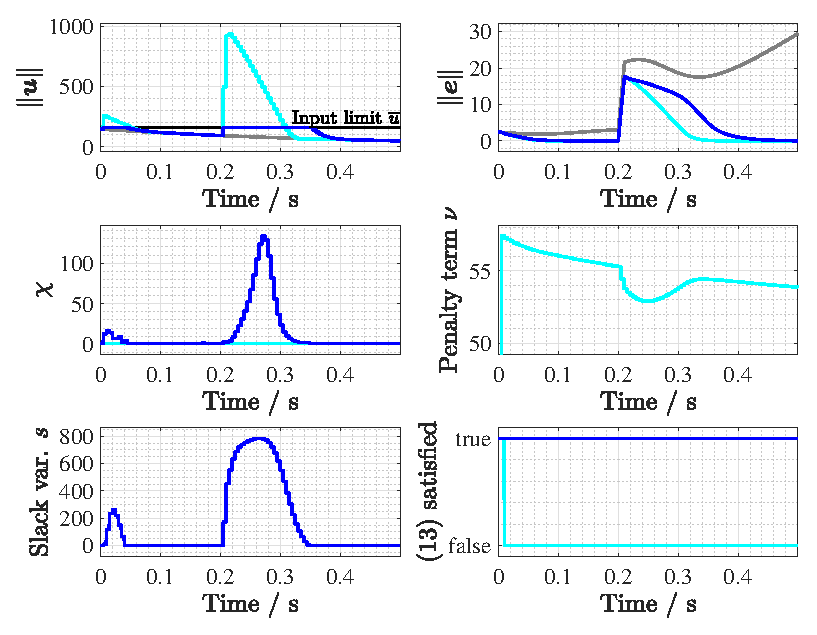
\includegraphics[width=0.99\linewidth]
      {
         src/figures/compare/Fig2.eps
      }
      \label{fig:sim:result:opt}
   }
   \caption{
      Numerical validation results of (C$_1$) \protect\colorLine{blue}{solid}, (C$_2$) \protect\colorLine{my_cyan}{solid}, (C$_3$) \protect\colorLine{gray}{solid}, and desired trajectory $x_d$ \protect\colorLine{red}{dashed}, and the saturated input of (C$_2$) \protect\colorLine{darkcyan}{solid}.
   }
   \label{fig:sim:result}
\end{figure}

% \begin{figure}[t]
%    \centering
%    \includegraphics[width=0.99\linewidth]
%    {
%       src/figures/compare/Fig1.eps
%    }
%    \caption{
%       Numerical validation results of (C$_1$) \protect\colorLine{blue}{solid}, (C$_2$) \protect\colorLine{my_cyan}{solid}, (C$_3$) \protect\colorLine{gray}{solid}, and desired trajectory $x_d$ \protect\colorLine{red}{dashed}.
%       The saturated input of (C$_2$) is indicated by \protect\colorLine{darkcyan}{solid} in the right-hand side figures
%    }
%    \label{fig:sim:result:control}
% \end{figure}

% \begin{figure}[t]
%    \centering
%    \includegraphics[width=0.99\linewidth]
%    {
%       src/figures/compare/Fig2.eps
%    }
%    \caption{
%       Control input norms, condition numbers, penalty term, and slack variable of (C$_1$) \protect\colorLine{blue}{solid}, (C$_2$) \protect\colorLine{my_cyan}{solid}, and (C$_3$) \protect\colorLine{gray}{solid}.
%    }
%    \label{fig:sim:result:opt}
% \end{figure}

\begin{table}[t]
   \renewcommand{\arraystretch}{1.5}
   \caption{Tracking performances in $L_2$ norm.}
   \centering
   \begin{tabular}{c c c c }
   % \begin{tabular}{c c c c c}
   \hline
   & (C$_1$) \protect\colorLine{blue}{solid} & (C$_2$) \protect\colorLine{my_cyan}{solid} & (C$_3$) \protect\colorLine{gray}{solid} \\
   \hline
   \hline 
   % \multirow{2}{*}{
   $\int_0^T\norm{\mv{e}}\,\der t$
   % } 
   & \oneErr & \twoErr & \threeErr \\
   % & (-\impOne \%)  & (-\impTwo \%) & (–) \\
   \hline
   \end{tabular}
   \label{table:performance}
\end{table}

The numerical validation results are illustrated in Fig.~\ref{fig:sim:result}.
When only the desired controller for nominal model, $\mv{u}=\mv{u}_d$, was applied, \ie (C$_3$), the trajectories of (C$_3$) and $\mv{x}_d$ do not coincide due to the effect of initial condition mismatch.
Significantly, after the disturbance occurrence at $t=0.2$ seconds, the trajectory deviates further from the desired trajectory, as shown in Fig.~\ref{fig:sim:result:control}.

By applying the contraction-based controllers, both (C$_1$) and (C$_2$) successfully drive the trajectory to closely follow the desired trajectory $\mv{x}_d$ even in the presence of disturbances, minimizing the $L_2$ norm of the tracking error to {\oneErr} and {\twoErr}, while (C$_3$) resulted in {\threeErr}, as summarized in Table~\ref{table:performance}.
However, regarding input saturation, (C$_2$) reaches the saturation limit due to the initial condition mismatch and the disturbance at $t=0.2$, while (C$_1$) effectively avoids input saturation, as shown in Fig.~\ref{fig:sim:result:opt}.
This demonstrates the effectiveness of the proposed method in handling input saturation constraints while achieving satisfactory tracking performance.

In addition, the expected behavior of the condition number $\chi$ of the contraction metrics, discussed in Section \ref{sec:sub:illustrative} and Fig.~\ref{fig:scene:first}, can be observed for (C$_1$) in Fig.~\ref{fig:sim:result:opt}.
As the contraction constraint \eqref{eq:cstr:ctrc} and the input saturation constraint \eqref{eq:cstr:sat} become active, the angle between $\mv{y}$ and $\mv{e}$ increases, resulting in an increase in the condition number to find an unsaturated optimal solution.
Specifically, when the input saturation constraint became active, the condition number $\chi$ increased from $1$ and decreased again to $1$ after the saturation effect disappeared.

In contrast, (C$_2$) shows the smallest condition number, $\chi=1$, due to the problem formulation issue discussed in Remark~\ref{rem:scale:invariance}.
Instead of adjusting the condition number, (C$_2$) increases the penalty term $\nu$ to increase the control effort, as shown in Fig.~\ref{fig:sim:result:opt}, while making $\overline{W}$ close to the identity matrix, \ie $\mm{M}=\nu\mm{I}_n$.
This results in the failure to satisfy the contraction constraint \eqref{eq:cstr:ctrc} during most of the simulation time, as shown in Fig.~\ref{fig:sim:result:opt}.

Despite achieving better $L_2$ tracking performance, (C$_2$) violated both the contraction constraint \eqref{eq:cstr:ctrc} and the input saturation limits as shown in Fig.~\ref{fig:sim:result:opt}.
These violations undermine stability guarantees, making the controller unsuitable for practical implementation.

\section{Conclusion} \label{sec:conclusion}

In this study, we presented a vector-space optimization framework for contraction metric calculation in contraction theory-based control design.
By projecting the contraction constraints onto the trajectory error vector space, the contraction metrics can be calculated in a lower-dimensional effective space, resolving the scalability issue of the conventional LMI framework.
The optimization problem was formulated to minimize the condition number of the contraction metric, where energy-based constraints were introduced to resolve the scale-invariance ambiguity and ensure sufficient control effort. 
Additionally, convex input saturation constraints were easily incorporated into the proposed framework owing to its flexibility of vector-space optimization problem compared to the matrix-space optimization of conventional LMI framework.
As future work, we will extend the proposed method to handle state constraints and validate it through real-world experiments.

The main advantage of the projected condition is that it reduces the online decision variable from a matrix-valued contraction metric to the metric-weighted error vector, which directly determines the feedback input. This reduction improves scalability and allows input constraints to be imposed more directly in the vector space. However, the projected condition is not equivalent to the full matrix-valued contraction condition. It enforces the contraction inequality only along the instantaneous trajectory-error direction and therefore guarantees a contraction-like decrease of the metric-weighted tracking-error energy, rather than full contraction of the closed-loop system.

% \begin{ack}
% Place acknowledgments here.
% \end{ack}

\bibliography{refs, localRefs}             % bib file to produce the bibliography
                                    % with bibtex (preferred)
\end{document}
